\documentclass[border=1.5pt]{standalone}
\usepackage{amsmath,amssymb}
\usepackage{tikz}
\usetikzlibrary{arrows.meta,calc,positioning,shapes,shapes.misc,shapes.geometric,backgrounds,fit,decorations.pathreplacing,quantikz2}
% Shared colors and styles for the XYZ^2 figures.
% Pauli types: bright tones for fills and bands, deep (800) shades of the same hues for labels.
% The label shades keep the hue of each Pauli, are well separated from each other (CIEDE2000 > 20)
% and have a contrast ratio of at least 2.9 on the coral cells and 4.5 on the sunflower cells.
\definecolor{PauliX}{HTML}{F97316}
\definecolor{PauliY}{HTML}{EC4899}
\definecolor{PauliZ}{HTML}{9333EA}
\definecolor{PauliXText}{HTML}{AC340B}
\definecolor{PauliYText}{HTML}{9D174D}
\definecolor{PauliZText}{HTML}{5B21B6}
% Generator classes: S0 (class B, even links, coral) and gauge (class A, odd links, sunflower)
\definecolor{Szero}{HTML}{F0435E}
\definecolor{SzeroText}{HTML}{BE123C}
\definecolor{Gauge}{HTML}{F59E0B}
\definecolor{GaugeText}{HTML}{B45309}
\colorlet{GaugeGray}{Gauge}
\definecolor{ClassB}{HTML}{FF8A99}
\definecolor{ClassA}{HTML}{FFD23F}
% Logical operators (X-bar violet, Z-bar crimson), errors, ink
\definecolor{LogicalZ}{HTML}{E11D48}
\definecolor{LogicalGold}{HTML}{7C3AED}
\definecolor{ErrRed}{HTML}{1C1917}
\definecolor{InkDark}{HTML}{292524}
\definecolor{InkSoft}{HTML}{57534E}
% Labels drawn on top of colored cells
\colorlet{CellText}{InkDark}
% Noise channels
\definecolor{ErrFlip}{HTML}{EF4444}
\definecolor{Idle}{HTML}{EC4899}
\definecolor{TwoQ}{HTML}{7C3AED}
% Protocol steps
\definecolor{StepPrep}{HTML}{F97316}
\definecolor{StepMeas}{HTML}{D946EF}
\definecolor{StepDec}{HTML}{7C3AED}
\definecolor{StepRec}{HTML}{DB2777}
\tikzset{
  qb/.style={circle, draw=InkDark, line width=0.6pt, fill=white,
             minimum size=4.2mm, inner sep=0pt, font=\scriptsize},
  qbsmall/.style={circle, draw=InkDark, line width=0.5pt, fill=white,
             minimum size=2.6mm, inner sep=0pt},
  hexedge/.style={line width=0.65pt, draw=InkSoft},
  linkedge/.style={line width=1.6pt, draw=InkDark},
  bndedge/.style={line width=0.65pt, draw=InkSoft, densely dashed},
  plabel/.style={font=\scriptsize\bfseries, inner sep=1pt},
  panel/.style={font=\small\bfseries, anchor=north west},
}

\providecommand{\ket}[1]{\left|#1\right\rangle}

\begin{document}
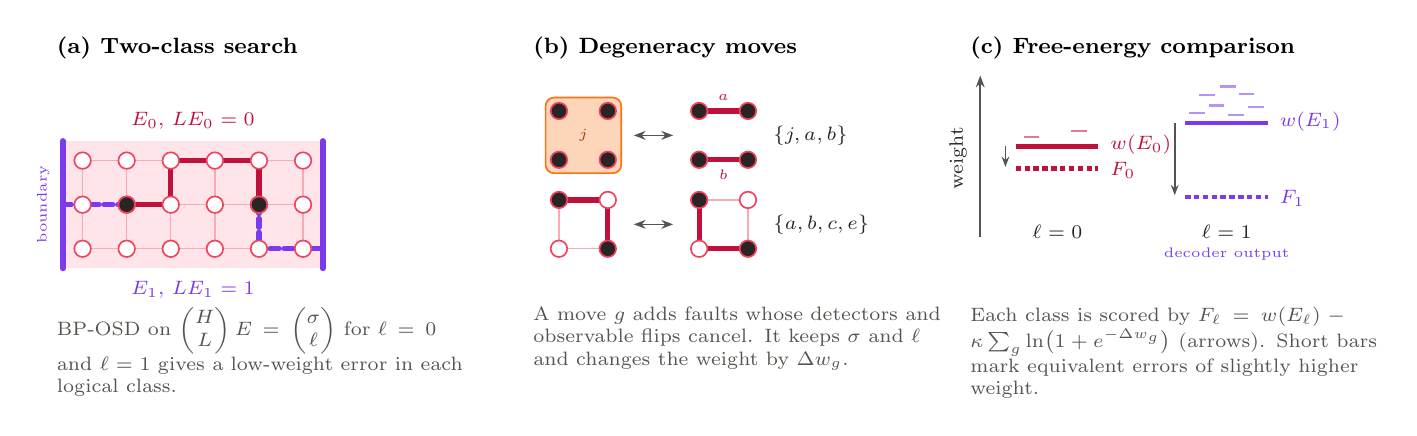
\begin{tikzpicture}[
  det/.style={circle, draw=Szero, line width=0.6pt, fill=white, minimum size=2.1mm, inner sep=0pt},
  lit/.style={circle, draw=Szero, line width=0.6pt, fill=InkDark, minimum size=2.1mm, inner sep=0pt},
  gridedge/.style={line width=0.45pt, draw=Szero!45},
  bnd/.style={line width=2.0pt, draw=LogicalGold, line cap=round},
  eA/.style={line width=1.9pt, draw=SzeroText, line cap=round},
  eB/.style={line width=1.9pt, draw=LogicalGold, line cap=round, dash pattern=on 3.2pt off 1.8pt},
  lab/.style={font=\scriptsize, text=InkDark},
  sub/.style={font=\scriptsize, text=InkSoft, align=left, anchor=north west, text width=5.2cm},
  title/.style={font=\footnotesize\bfseries, anchor=west},
]
\def\s{0.56}
% =========================================================== (a) two-class search
\begin{scope}[shift={(0,0)}]
  \node[title] at (-0.45,2.55) {(a) Two-class search};
  \fill[ClassB!22] (-0.25,-0.25) rectangle (5*\s+0.25,2*\s+0.25);
  \foreach \i in {0,...,5} \foreach \j in {0,1,2} {
    \ifnum\i<5 \draw[gridedge] (\i*\s,\j*\s) -- ({(\i+1)*\s},\j*\s); \fi
    \ifnum\j<2 \draw[gridedge] (\i*\s,\j*\s) -- (\i*\s,{(\j+1)*\s}); \fi
  }
  \draw[bnd] (-0.25,-0.25) -- (-0.25,2*\s+0.25);
  \draw[bnd] (5*\s+0.25,-0.25) -- (5*\s+0.25,2*\s+0.25);
  % E_0 : connects the two detection events
  \draw[eA] (1*\s,1*\s) -- (2*\s,1*\s) -- (2*\s,2*\s) -- (3*\s,2*\s) -- (4*\s,2*\s) -- (4*\s,1*\s);
  % E_1 : each detection event to a boundary
  \draw[eB] (1*\s,1*\s) -- (0,1*\s) -- (-0.25,1*\s);
  \draw[eB] (4*\s,1*\s) -- (4*\s,0) -- (5*\s,0) -- (5*\s+0.25,0);
  \foreach \i in {0,...,5} \foreach \j in {0,1,2} {\node[det] at (\i*\s,\j*\s) {};}
  \node[lit] at (1*\s,1*\s) {};
  \node[lit] at (4*\s,1*\s) {};
  \node[lab, text=SzeroText, anchor=south] at (2.5*\s,2*\s+0.27) {$E_0$, $L E_0=0$};
  \node[lab, text=LogicalGold, anchor=north] at (2.5*\s,-0.29) {$E_1$, $L E_1=1$};
  \node[font=\tiny, text=LogicalGold, rotate=90, anchor=south] at (-0.3,1*\s) {boundary};
  \node[sub] at (-0.45,-0.62) {BP-OSD on $\begin{pmatrix}H\\ L\end{pmatrix}E=\begin{pmatrix}\sigma\\ \ell\end{pmatrix}$ for $\ell=0$ and $\ell=1$ gives a low-weight error in each logical class.};
\end{scope}
% =========================================================== (b) degeneracy moves
\begin{scope}[shift={(6.05,0)}]
  \node[title] at (-0.45,2.55) {(b) Degeneracy moves};
  % --- three-fault move: hyperedge j = a + b
  \coordinate (A) at (0,1.75); \coordinate (B) at (0.62,1.75);
  \coordinate (C) at (0,1.13); \coordinate (D) at (0.62,1.13);
  \fill[PauliX!30, draw=PauliX, line width=0.6pt, rounded corners=3pt] ($(A)+(-0.17,0.17)$) rectangle ($(D)+(0.17,-0.17)$);
  \node[font=\tiny, text=PauliXText] at ($(A)!0.5!(D)$) {$j$};
  \foreach \p in {A,B,C,D} {\node[lit] at (\p) {};}
  \draw[{Stealth[length=1.5mm]}-{Stealth[length=1.5mm]}, line width=0.6pt, draw=InkSoft] (0.95,1.44) -- (1.45,1.44);
  \coordinate (A2) at (1.78,1.75); \coordinate (B2) at (2.4,1.75);
  \coordinate (C2) at (1.78,1.13); \coordinate (D2) at (2.4,1.13);
  \draw[eA] (A2) -- (B2) node[midway, above=-0.5pt, font=\tiny, text=SzeroText] {$a$};
  \draw[eA] (C2) -- (D2) node[midway, below=-0.5pt, font=\tiny, text=SzeroText] {$b$};
  \foreach \p in {A2,B2,C2,D2} {\node[lit] at (\p) {};}
  \node[lab, anchor=west] at (2.6,1.44) {$\{j,a,b\}$};
  % --- four-fault move: two paths around a square
  \coordinate (P) at (0,0.62); \coordinate (Q) at (0.62,0.62);
  \coordinate (R) at (0.62,0); \coordinate (S) at (0,0);
  \draw[gridedge] (P) -- (S) -- (R);
  \draw[eA] (P) -- (Q) -- (R);
  \foreach \p in {P,R} {\node[lit] at (\p) {};}
  \foreach \p in {Q,S} {\node[det] at (\p) {};}
  \draw[{Stealth[length=1.5mm]}-{Stealth[length=1.5mm]}, line width=0.6pt, draw=InkSoft] (0.95,0.31) -- (1.45,0.31);
  \coordinate (P2) at (1.78,0.62); \coordinate (Q2) at (2.4,0.62);
  \coordinate (R2) at (2.4,0); \coordinate (S2) at (1.78,0);
  \draw[gridedge] (P2) -- (Q2) -- (R2);
  \draw[eA] (P2) -- (S2) -- (R2);
  \foreach \p in {P2,R2} {\node[lit] at (\p) {};}
  \foreach \p in {Q2,S2} {\node[det] at (\p) {};}
  \node[lab, anchor=west] at (2.6,0.31) {$\{a,b,c,e\}$};
  \node[sub] at (-0.45,-0.62) {A move $g$ adds faults whose detectors and observable flips cancel. It keeps $\sigma$ and $\ell$ and changes the weight by $\Delta w_g$.};
\end{scope}
% =========================================================== (c) free energies
\begin{scope}[shift={(11.6,0)}]
  \node[title] at (-0.45,2.55) {(c) Free-energy comparison};
  \draw[-{Stealth[length=1.5mm]}, line width=0.6pt, draw=InkSoft] (-0.2,0.15) -- (-0.2,2.2);
  \node[lab, rotate=90, anchor=south] at (-0.25,1.15) {weight};
  % class 0: small entropy
  \foreach \x/\y in {0.45/1.42,1.05/1.5} {\draw[line width=0.8pt, draw=SzeroText!55] (\x-0.1,\y) -- (\x+0.1,\y);}
  \draw[line width=1.6pt, draw=SzeroText] (0.25,1.3) -- (1.3,1.3);
  \draw[line width=1.6pt, draw=SzeroText, dash pattern=on 2pt off 1.2pt] (0.25,1.02) -- (1.3,1.02);
  \draw[-{Stealth[length=1.3mm]}, line width=0.6pt, draw=InkSoft] (0.12,1.3) -- (0.12,1.04);
  \node[lab, text=SzeroText, anchor=west] at (1.33,1.32) {$w(E_0)$};
  \node[lab, text=SzeroText, anchor=west] at (1.33,1.0) {$F_0$};
  % class 1: large entropy
  \foreach \x/\y in {2.55/1.72,2.8/1.82,3.05/1.7,3.3/1.8,2.68/1.95,3.18/1.97,2.95/2.06} {\draw[line width=0.8pt, draw=LogicalGold!55] (\x-0.1,\y) -- (\x+0.1,\y);}
  \draw[line width=1.6pt, draw=LogicalGold] (2.4,1.6) -- (3.45,1.6);
  \draw[line width=1.6pt, draw=LogicalGold, dash pattern=on 2pt off 1.2pt] (2.4,0.66) -- (3.45,0.66);
  \draw[-{Stealth[length=1.3mm]}, line width=0.6pt, draw=InkSoft] (2.27,1.6) -- (2.27,0.68);
  \node[lab, text=LogicalGold, anchor=west] at (3.48,1.62) {$w(E_1)$};
  \node[lab, text=LogicalGold, anchor=west] at (3.48,0.64) {$F_1$};
  \node[lab, anchor=north] at (0.78,0.42) {$\ell=0$};
  \node[lab, anchor=north] at (2.93,0.42) {$\ell=1$};
  \node[font=\tiny, text=LogicalGold, anchor=north] at (2.93,0.14) {decoder output};
  \node[sub] at (-0.45,-0.62) {Each class is scored by $F_\ell=w(E_\ell)-\kappa\sum_g\ln\!\big(1+e^{-\Delta w_g}\big)$ (arrows). Short bars mark equivalent errors of slightly higher weight.};
\end{scope}
\end{tikzpicture}

\end{document}
